\chapter{Exponential integration methods in JAGUAR}

  \paragraph{}
  We want to analyse time exponential integration methods in a framework that gives us access to high-order spatial discretisation methods.
  It is possible to use high-order Finite Volume methods, but this means using larger stencils which hurts parallelism.
  In CEDRE, users often stop at second-order methods, so we need to use another solver.
  As the spatial discretisation method does not play a direct role in the time integration and the work done in this thesis, we can step out from the Finite Volume framework.
  Furthermore, using a less complex solver will also help us try and develop new methods more easily than we already did with CEDRE.
  This is why we decided to accomplish our analysis of exponential time integration methods with the solver JAGUAR.


  \section{JAGUAR: a Spectral Difference solver}

    \paragraph{}
    JAGUAR means proJect of an Aerodynamic solver using General Unstructured grids And high ordeR schemes.
    It is a reactive Navier--Stokes solver initially developed at the European center for research and advanced training in scientific computing: CERFACS.
    It is made for unstructured grids and uses a Large Eddy Simulation model to solve turbulence.
    Its particularity is that it uses a spectral method as the spatial discretisation scheme: the Spectral Difference method.


    \subsection{The Spectral Difference method}

      \paragraph{}
      With the Spectral Difference method, the solution is represented by a polynomial of degree $p$ inside each cell.
      It means that in the partial differential equation
      \begin{equation}\label{eq:pde_2}
        \frac{\partial u}{\partial t} + \nabla \cdot F\left(u\right) = 0 \ ,
      \end{equation}
      $u$ is a $p$-degree polynomial of the coordinate variables, where the polynomial coefficients are functions of time.
      Then $F\left(u\right)$ has to be a $p\!+\!1$-order polynomial of the coordinate variables.
      The key to the Spectral Difference method is how to compute a $p + 1$-order $F\left(u\right)$ from a $p$-order $u$.
      This method uses key elements that were first mentioned by \cite{Kopriva1996}, and was later developed by \cite{LiuVinokurWang2006}.

      \begin{figure}
        \centering
        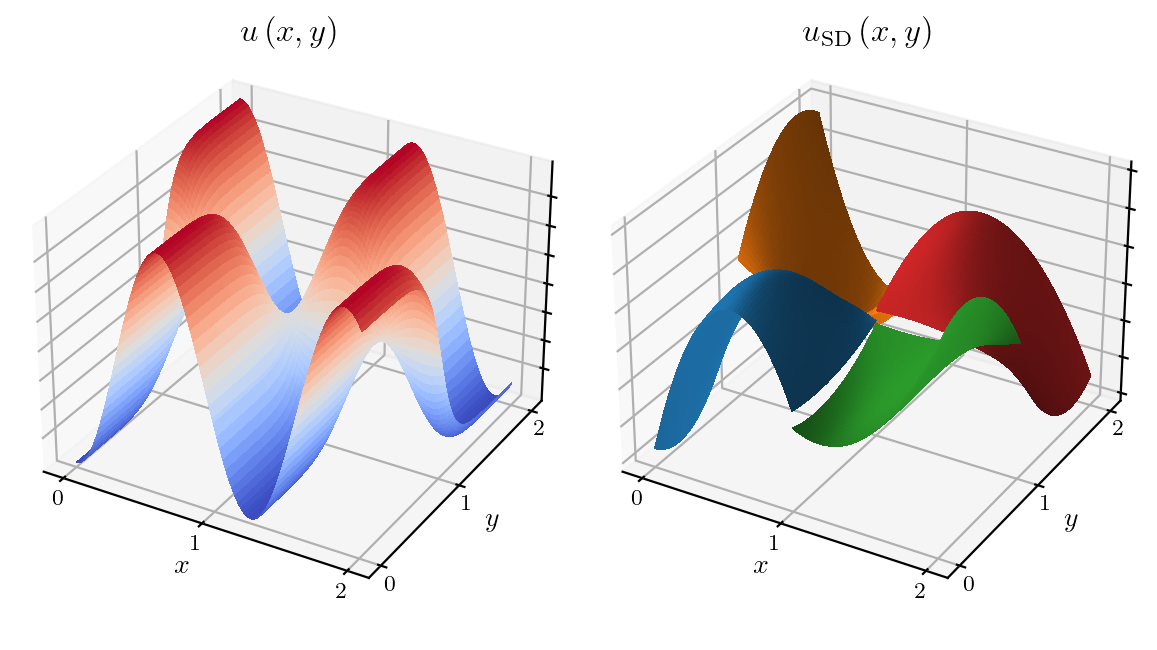
\includegraphics{figures/sd_discontinuous.png}
        \caption{Continuous function (left) and discontinuous representation made by the Spectral Difference method (right).}
        \label{fig:sd_discontinuous}
      \end{figure}

      \paragraph{}
      Because the solution is represented in each cell by a polynomial, there is no reason for the solution to be continuous throughout cell interfaces.
      Indeed, the Spectral Difference method uses a piecewise representation of the solution.
      For example, we show in figure \ref{fig:sd_discontinuous} a function represented as the Spectral Difference method represents the solution.
      The two-dimensional mesh is regular and made of $2 \times 2$ cells over $\left[0, 2\right]^2$.
      We represent the function
      \begin{equation}
        \begin{aligned}
          u \colon \left[0, 2\right]^2 &\to \mathbb{R}\\
          \left(x, y\right) &\mapsto \cos\left(5x\right) \tanh\left(5\left(1 - y\right)\right)
        \end{aligned}
      \end{equation}
      over the mesh in the left part of figure \ref{fig:sd_discontinuous}.
      The colour mapping corresponds to the output of the function but is not given as this function is of no particular interest, but is just an example for the point we make here.
      This function is interpolated with a second-order method using Lagrange polynomials over each cell.
      The result is shown in the right part of figure \ref{fig:sd_discontinuous}, where each colour corresponds to one cell.
      We see that there are discontinuities at the cell interfaces, which shows a specificity of the Spectral Difference methods.
      If we were to use the function on the left part of figure \ref{fig:sd_discontinuous} as an initial condition for a simulation, the Spectral Difference method would in fact use the function on the right part of the figure.
      However, to respect the underlying conservation property of equation (\ref{eq:pde_2}), it is necessary for $F$ to be continuous over the whole computational domain.
      The Spectral Difference method will then make sure that the polynomial representations of the flux density are continuous throughout cell interfaces.

      \paragraph{}
      To better understand how this method works, we take a one-dimensional cell: the segment $\left[0, 1\right]$.
      Because the following is done at a fixed time we will drop the dependency on the time, but the solution and the coefficients are in reality functions of the time, not scalars.
      The solution $u$ inside this segment is then $u\left(x\right) = \sum_{i=0}^p a_ix^i$.
      Using Lagrange interpolation polynomials, it is equivalent to use the set of the $p + 1$ coefficients $a_i$ or the set of the $p + 1$ values $u\left(x_i\right)$ computed at the distinct points $x_i \in \left[0, 1\right]$ called \emph{solution points}.
      The solution as a $p$-order polynomial is represented by either one of those two sets.
      As the flux density $F$ must be a $p\!+\!1$-order polynomial, it can also be represented by its values in the $p + 2$ distinct \emph{flux points}.
      To ensure that $F$ is continuous at the segment end points, we take $0$ and $1$ as flux points.
      The choice of the rest of the flux points will be discussed later, but let us say for now that they are staggered with the solution points: each flux point, apart from the segment end points, is between two solution points and vice versa.

      \begin{figure}
        \centering
        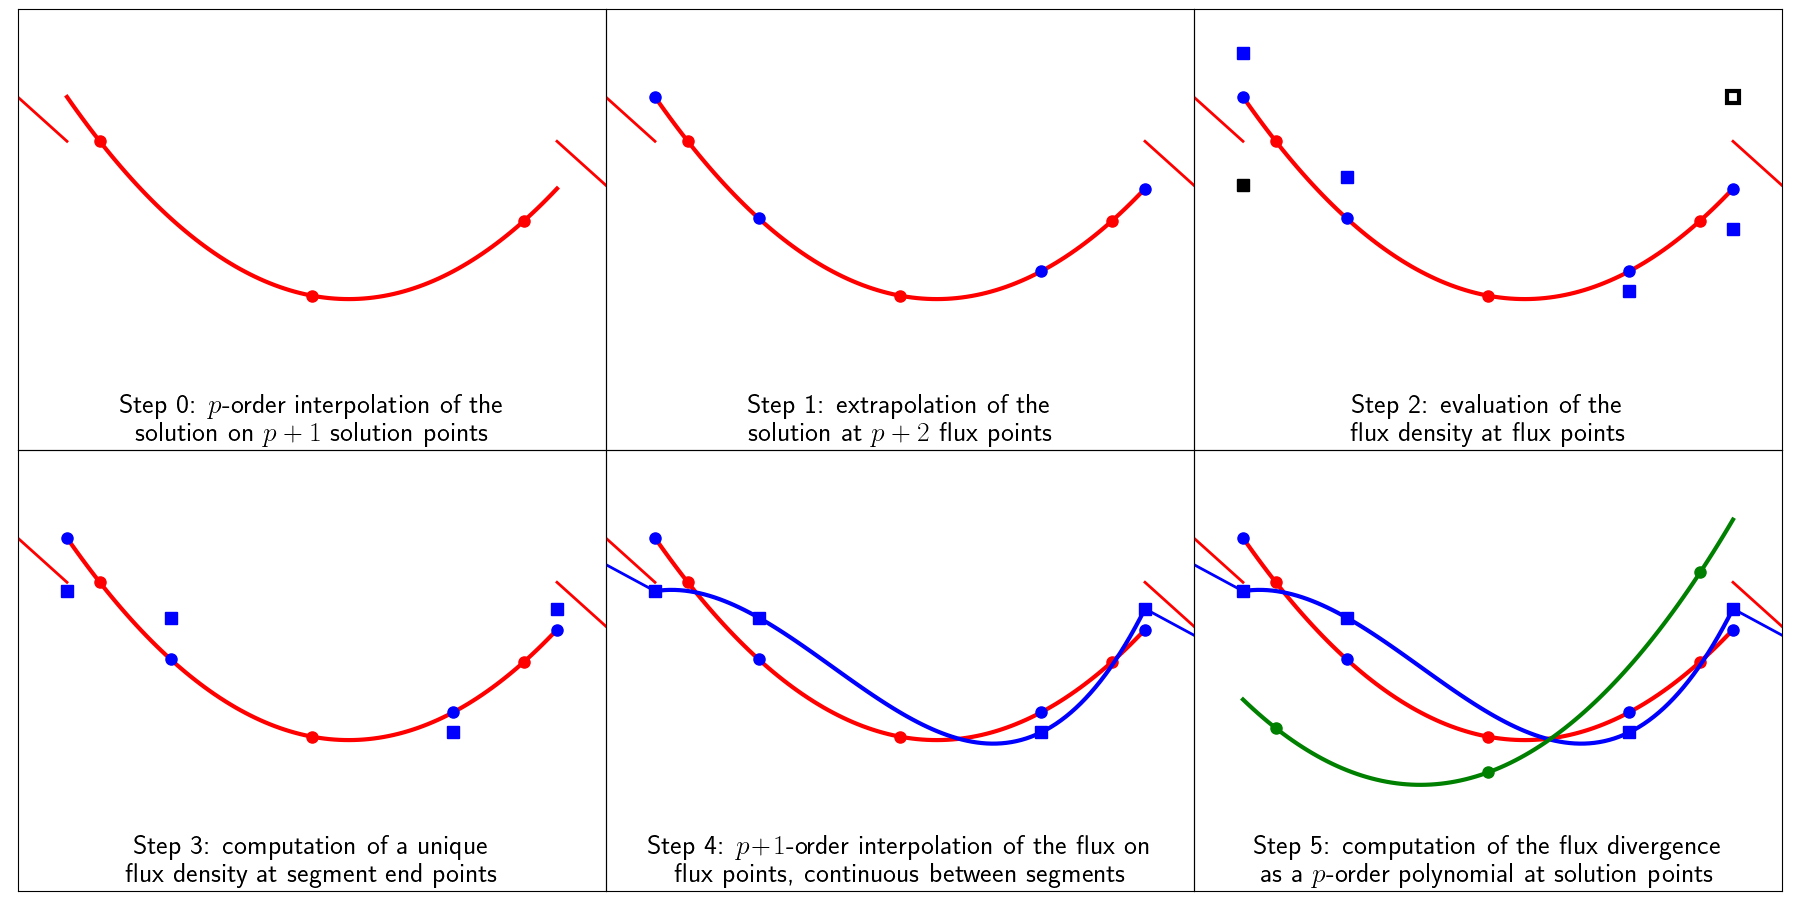
\includegraphics{figures/sd_scheme.png}
        \caption{Steps of the Spectral Difference methods with $p = 2$.}
        \label{fig:sd_scheme}
      \end{figure}

      \paragraph{}
      Figure \ref{fig:sd_scheme} shows the steps the Spectral Difference make to compute the flux divergence $\nabla \cdot F\left(u\right)$ from the solution $u$.
      In this example, we have $p = 2$.
      \begin{enumerate}
        \setcounter{enumi}{-1}
        \item At first, the solution is represented with a red line by its value in the $p + 1$ solution points.
        The solution points are marked by red dots.
        We see parts of the solution from the left and right neighbouring cells.
        As the figure shows and as we discussed before, they may be discontinuous from the solution in this cell.
        This is the starting point of the Spectral Difference method so we will call it the 0-th step.
        \item In the first step, the method computes the value of the solution in the $p + 2$ flux points, marked by blue dots.
        As the polynomial representing the solution is known, this step just consists in evaluating it at flux points.
        \item In the second step, the method evaluates the flux density $F\left(u\right)$ in each flux point.
        This is possible because we computed the solution in those points in the previous step.
        The values of the flux density are marked by blue squares in the figure.
        However, segment end points are flux points for the two neighbouring cells, and therefore we show in the figure a full black square for the flux at $0$ from the left neighbouring cell and an empty black square for the flux at $1$ from the right neighbouring cell.
        \item Because there are different values of the flux density at the segment end points, the method would not preserve the conservative property of the partial differential equation.
        This is why in the third step, the method computes a unique interface flux density for both cells at each segment end points.
        The problem is to find the interface flux at the discontinuity of a piecewise solution.
        In other words, this is a Riemann problem.
        Once again, this is solved with a Riemann solver, exact or approximate, to get in the end a single value for the left and right parts of the discontinuity.
        \item Now that we have the value of the flux density at the $p+2$ flux points, we can interpolate it with Lagrange polynomials to get a $p+1$ order $F$ as expected in the fourth step, represented with a blue line in the figure.
        We end up with a continuous representation of $F$, differentiable everywhere except at cell interfaces.
        \item In the last step, we can differentiate the representation of $F$ to get the flux divergence, represented by a green line in the figure.
        We finally get a $p$-order representation of $\nabla \cdot F$ that we can evaluate at the solution points.
      \end{enumerate}

      \paragraph{}
      To work with any segment, not only $\left[0, 1\right]$, we use an isoparametric transformation to get back to this unity segment.
      It is the same when working with multiple dimensions, where the isoparametric transformation gets the cell back to the tensor powers of this segment.
      The placement of the solution points does not seem to matter much, but the placement of the flux points does \cite{VandenAbeeleLacorWang2008}.
      The $p + 1$ solution points we will use are defined in the $\left[0, 1\right]$ segment as the Chebyshev roots:
      \begin{equation}
        x_i = \frac{1}{2} \left(1 - \cos\left(\frac{2i + 1}{2p + 2} \pi\right)\right), \quad, 0 \leq i \leq p \ .
      \end{equation}
      They are traditionally defined inside the $\left[-1, 1\right]$ segment but are scaled into $\left[0, 1\right]$.
      They are the roots of the Chebyshev polynomials of the first kind and are often used in polynomial interpolation as they tend to minimise Runge's phenomenon.
      The $p + 2$ flux points used by our methods are the $p$ roots of the $p$-th Legendre polynomials to which are added the two segment end points.
      This choice has the property that there is a flux point between each contiguous solution point.
      There is no explicit formula for the Legendre polynomial roots as there is one for the Chebyshev polynomial roots.
      Their value is taken from tables from the literature \PS{ref ?}.
      They are also defined in the $\left[-1, 1\right]$ segment and are scaled into $\left[0, 1\right]$.
      Finally, the solution and flux points can be seen in figure \ref{fig:sd_points}.

      \begin{figure}
        \centering
        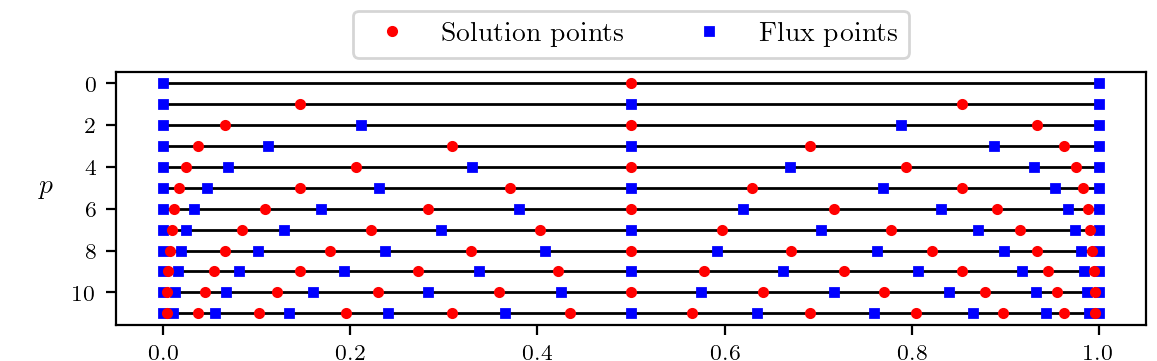
\includegraphics{figures/sd_points.png}
        \caption{Solution points and flux points in the $\left[0, 1\right]$ segment used in the Spectral Difference method for $0 \leq p \leq 11$.}
        \label{fig:sd_points}
      \end{figure}

      \paragraph{}
      As a side note, we see that the Spectral Difference method with $p = 0$ corresponds to the first-order Finite Volume method.
      Indeed, the solution is assumed constant in the cell, represented by the value at its barycenter.
      The flux balance is made at the cell interfaces with a Riemann solver.
      This corresponds to the placement of the solution and flux points in figure \ref{fig:sd_points} when $p = 0$.
      For higher $p$ we have a true Spectral Difference method, of order $p$ \PS{preuve de l'ordre ?}.
      In JAGUAR, we can chose the order $p$ from 2 to 10 \PS{10 en pratique ?}.


    \subsection{Exponential integration methods in JAGUAR}

      \paragraph{}
      We now have a high-order spatial discretisation method, so that when we test our high-order time integration methods the resulting error will come mostly from the time integration and not the spatial discretisation.
      The development of an exponential time integration method was inexpensive within CEDRE as the method reuses lots of already existing parts.
      For JAGUAR which only has explicit methods, we would have to develop the Arnoldi iteration in addition to the exponential computation functions.
      As this work does not aim to produce a finely tuned method for JAGUAR but to analyse scientifically exponential methods, we decided to rely on the SLEPc library \cite{HernandezRomanVidal2005}.
      The Scalable Library for Eigenvalue Problem Computation, or SLEPc, is an extension of the software library PETSc \cite{petsc-web-page, petsc-user-ref, petsc-efficient}.
      Instead of rewriting the algorithms we need, we can use their SLEPc implementation.
      In particular, SLEPc handles what it calls \emph{Matrix Function} objects or MFN:
      \begin{quote}
        "Given a matrix $A$ and a vector $b$, the call \mintinline{c}{MFNSolve(mfn, b, x)} computes \\
        $x=f\left(A\right) b$, where $f$ is a function such as the exponential."
      \end{quote}
      This is precisely what we need to develop our methods:
      As it handles the previously introduced $\varphi$-functions with its MFN objects, SLEPc is then an obvious choice of a library for implementing exponential integration methods.
      Furthermore, because it relies on PETSc, it is efficiently scalable to fit our multiprocessing needs.

      \paragraph{}
      We saw that exponential methods are based on a decomposition of the ordinary differential equation such as equation (\ref{eq:ode_split}).
      However, JAGUAR uses only explicit time integration methods, so no Jacobian matrix is available.
      Computing analytically the Jacobian matrix would prove challenging as we would have to differentiate the Spectral Difference scheme, the Riemann solvers, the diffusion scheme, etc.
      It is not insurmountable but would amount to more work than what we can afford during this thesis.
      We decided instead to reuse the work from the previous part: the Jacobian matrix will not be formed, but its effect will be computed by a finite difference approximation.
      Another reason to work with the SLEPc library is that using a finite difference approximation is easy with it.
      More precisely, it is PETSc that handles this approximation.
      To sum up, to compute $\varphi_k\left(L\right)b$ that is required for our exponential methods with $L = f'\left(y\right)$, we first use the fact that $L$ is a Jacobian matrix to create it with the appropriate PETSc data type.
      We only need to indicate to PETSc what function $L$ it is the Jacobian matrix of, that is $f$.
      Then, after setting the MFN object of SLEPc, we can compute the desired result.
      The Arnoldi iteration, the Scaling and Squaring algorithm and the exponential evaluation are all handled internally by the library.
      Overall, this procedure is extremely simple from our perspective and requires only a few lines of code to implement.
      This highlight the relevance of using the SLEPc library.

      \paragraph{}
      With what we described, we are able to write an exponential time integration method in JAGUAR.
      Other people that also work with JAGUAR did develop implicit time integration methods using PETSc.
      To continue in this direction, we decided to add a time integration method based on the generic PETSc Time Stepper \cite{AbhyankarBrownConstantinescuEtAl2018}.
      This way, a user may use most methods from PETSc in JAGUAR with no additional developments
      It includes any explicit and implicit time integration methods, but also nonlinear solvers such as Newton's methods with various line search algorithms, linear solvers with various Krylov subspace methods and finally various preconditioning.
      However, this generic PETSc Time Stepper method was added on the side of this thesis, and therefore will not be discussed here, along with the previous work on implicit methods.


    \paragraph{}
    In the end, we now have a high-order spatial discretisation method with the Spectral Difference method that allows us to analyse and compare exponential methods.
    In the following, we will work with the three methods we developed in JAGUAR and we presented earlier in table \ref{tab:exprb_butcher}: the Rosenbrock--Euler, ExpRB32 and ExpRB42 methods.


  \section{Analysis of exponential time integration methods}

    \paragraph{}
    We now have in JAGUAR all the tools necessary to analyse exponential time integration methods.
    We have to choose several test cases to do so.
    We compare the exponential methods to explicit Runge--Kutta methods as they are the only available methods in JAGUAR.
    Those methods are:
    \begin{itemize}
      \item RK2, the Midpoint method
      \item RK4, the classical four-stage fourth-order method
      \item RKo6s, a low-storage six-stage second-order method from \cite{BogeyBailly2004}
      \item TVDRK(3, 3), a three-stage third-order TVD method from \cite{ShuOsher1988, GottliebShu1996}
      \item SSPRK(5, 4), an optimal SSP five-stage fourth-order method from \cite{SpiteriRuuth2002}.
    \end{itemize}
    Low-storage methods are Runge--Kutta methods for which the matrix $A$ in their Butcher tableau is lower diagonal, or in other words all $a_{ij}$ are null except when $j = i - 1$.
    Also, all $b_i$ are null except the last one that is equal to $1$.
    It means that the final stage and all intermediate ones use only the previous stage.
    Therefore we do not need to keep track of the intermediate stages in memory, only to update the current value, which gives the name low-storage method.
    The last two methods are Runge--Kutta methods with an additional property originally called TVD \cite{GottliebShu1996} and more recently SSP  \cite{GottliebShuTadmor2001}.
    Without going into too much detail, it means that they are methods that are convex combinations of explicit Euler steps so that their stability is guaranteed for sufficiently small time steps.
    To us, it means they are defined differently than other methods, using the coefficients $\alpha_{0 < i \leq k, 0\leq j < i}$ and $\beta_{0 < i \leq k, 0\leq j < i}$ as:
    \begin{equation}
      \left\{\begin{aligned}
        y_{n+1} &= y^{\left(k\right)} \\
        \textrm{with}\quad y^{\left(i\right)} &= \sum_{j = 0}^{i-1} \alpha_{ij} y^{\left(j\right)} + \Delta t \beta_{ij} f\left(y^{\left(j\right)}\right) , \quad 1 \leq i \leq k\\
        \textrm{and}\quad y^{\left(0\right)} &= y_n
      \end{aligned}\right. \ .
    \end{equation}
    However, they are equivalent to traditional Runge--Kutta methods in the sense that they can be represented by the standard Butcher tableau, with:
    \begin{equation}
      \left\{\begin{aligned}
        a_{ij} &= \sum_{l = j+1}^{i-1} \alpha_{i-1, l-1} a_{l, j} + \beta_{i-1, j-1} \\
        b_i &= \sum_{l = i+1}^{k} \alpha_{k, l-1} a_{l, i} + \beta_{k, i-1}
      \end{aligned}\right. \ .
    \end{equation}
    We can finally say that we are indeed working with explicit Runge--Kutta methods, as they were introduced initially.


    \subsection{Order: convected inviscid isentropic vortex}

      \paragraph{}
      For the first test, we wanted to see if the orders of the exponential time integration methods were the correct ones when used in JAGUAR.
      We decided to use the same test case we used with CEDRE: the two-dimensional inviscid isentropic vortex.
      The case is still described by equation \ref{eq:covo}, but the numerical values are different.
      The convective flow Mach number is still $0.5$, but this time $P_\infty = 10^5$ and $T_\infty = 300$.
      The heat capacity ratio is $\gamma = 1.4$ and the specific gas constant is $r_\textrm{gas} = 287.058$.
      The mesh represent the two-dimensional box $\left[0, L\right]^2$ with $L = 0.1$, and is made of $N \times N$ cells.
      The vortex is defined by its characteristic radius $R_0 = 0.005$ and its intensity $\beta = 0.2$.
      It corresponds in fact to the same vortex as the one we used with CEDRE, in size and in intensity, but it has been scaled down into a smaller box and dimensioned to some given pressure and temperature.
      \PS{unités ?}

      \paragraph{}
      The period for those numerical values is \PS{TODO}.
      After 20 periods, we can compute the $L_2$ error for a scalar variable $u\left(\vec{x}, t\right)$:
      \begin{equation}
        \operatorname{err}\left(u\right) = \left(\int_{\left[0, L\right]^2} \left(u\left(\vec{x}, 20T\right) - u\left(\vec{x}, 0\right)\right)^2 \mathrm{d}\vec{x} \right)^{1/2} \ .
      \end{equation}
      Because it is a periodic case, the initial value corresponds to the exact solution.
      This error corresponds then to the error of the time integration method.
      By looking at this error as a function of the time step, we can determine the order of our time integration methods.

      \paragraph{}
      The error we get is the global truncation error: the error the method makes while getting to a fixed time, no matter how many iterations it took.
      However, we previously defined the order of a time integration method using the local truncation error: the error it makes after a single small step.
      There is a link between global and local truncation errors for our single-step methods.
      Let us call $\tau_n$ the local truncation error and $e_n$ the global truncation error at step $n$.
      Because our methods are single-step methods that can be written as:
      \begin{equation}
        y_{n+1} = y_n + \Delta t_n g\left(y_n, \Delta t_n\right) \ ,
      \end{equation}
      with an increment function $g$ that is $K$-Lipschitz continuous in the $y$ variable, we have \cite{SueliMayers2003}:
      \begin{equation}
        \left| e_n \right| \leq \frac{\max_{1 \leq i \leq n} \left| \tau_i \right|}{K \Delta t_n} \left(e^{K\left(t_n - t_0\right)} - 1\right) \ .
      \end{equation}
      A method is a $p$-order method if $\tau_n = O\left(\Delta t^{p+1}\right)$.
      Therefore, a $p$-order method verify $e_n = O\left(\Delta t^{p}\right)$.
      However, the reciprocal is not true: just because we observe a global truncation error is $e_n = O\left(\Delta t^{p}\right)$ does not mean the order of the method is $p$.
      Here we do not look at the error to show the method orders are correct, but to see if we end up with the expected order for the global truncation error, as it is the error users look at.
      The proof of the order for a method is analytical, by writing the partial Taylor series of the exact solution, as we did earlier for the exponential Rosenbrock--Euler method.

      \paragraph{}
      The point of this analysis is to see how the global truncation error depends on the time step $\Delta t$ that is kept constant throughout the computations.
      Because some methods are more accurate than others, we did several computations with different mesh resolutions and Spectral Difference method orders.
      We start with the Midpoint method.
      We take the order of the spatial discretisation method $p = 4$.
      We look at the $L_2$ error for the pressure after 20 periods, for given time steps.
      We will in fact show results using the CFL number, as it is proportional to the time step:
      \begin{equation}
        \mathcal{N}_\textrm{CFL} = \frac{N \left(p + 1\right) \left(1 + \operatorname{Ma}\right) \sqrt{\gamma r_\textrm{gas} T}}{L} \Delta t\ .
      \end{equation}
      Using the CFL number instead of the time step allows us to compare results with different $N$ or even $p$.
      It can be seen here as a nondimensional time.
      We do the computation for multiple values of $N$: 16, 32 and 64.
      The result is shown in figure \ref{fig:covo_rk2}.
      We see that the $16\times16$ mesh does not allow for a good analysis: the error due to the spatial discretisation method is too important and prevents us to see the expected dependency between the global truncation error and the time step.
      The two other meshes however show the expected relation: $\operatorname{err} = O\left(\Delta t^2\right)$.

      \begin{figure}
        \centering
        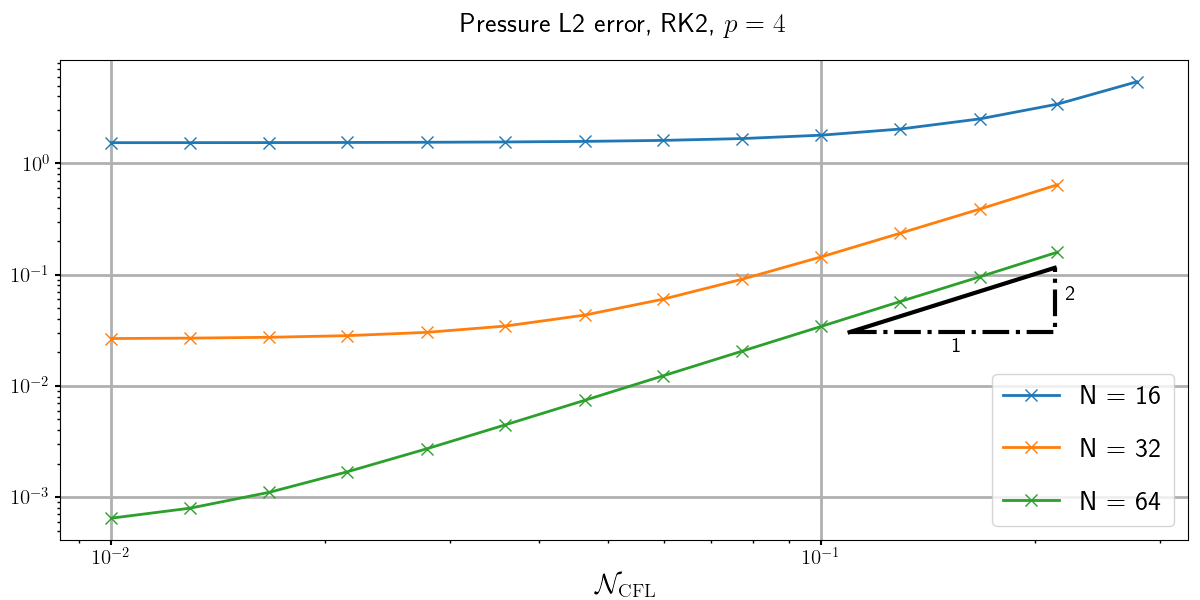
\includegraphics{figures/covo_rk2.png}
        \caption{Global truncation error for the RK2 Midpoint method.}
        \label{fig:covo_rk2}
      \end{figure}

      \paragraph{}
      We can repeat this analysis for other methods, and we look next at the RK4 method.
      However, we see in figure \ref{fig:covo_rk2_rk4} that the error is constant no matter the value of $N$.
      It is because the error due to the RK4 method is so small that it is dominated by the error due to the spatial discretisation scheme.
      It is useless to do the same for lower time steps, as the error would not change, therefore the RK4 error lines are continued by black dashed lines.
      We still see the curves corresponding to the Midpoint method.
      As the time step decreases, we see that those curves tend to the dashed lines: to the same values as the constant errors we have with the RK4 method.
      This lower bound for the error corresponds to the error of the Spectral Difference method.
      It shows once again that we need spatial discretisation methods with small errors in order to analyse time integration methods.

      \begin{figure}
        \centering
        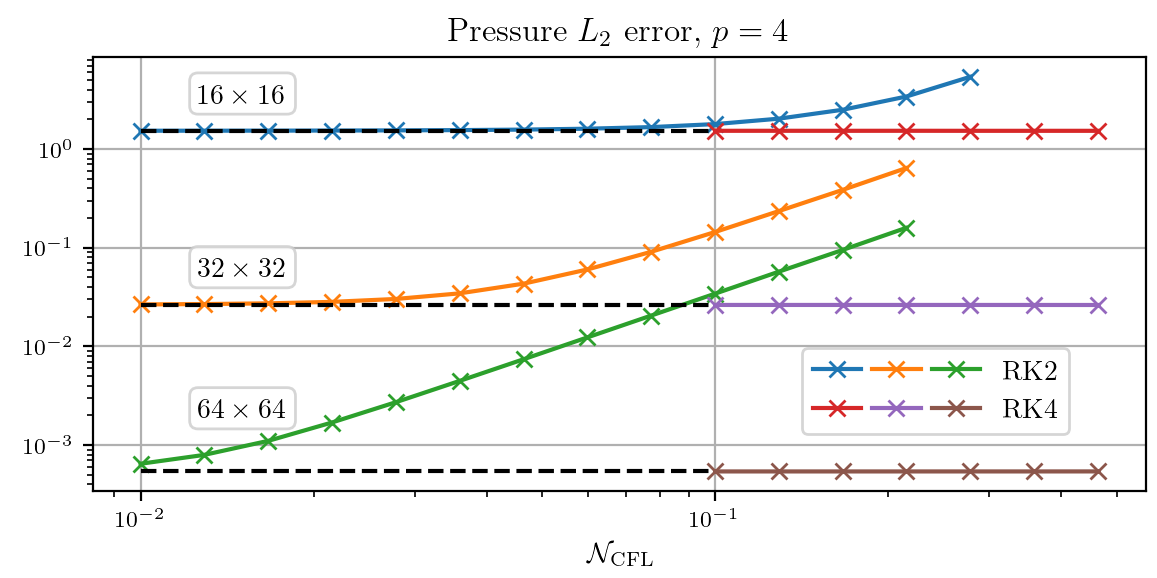
\includegraphics{figures/covo_rk2_rk4.png}
        \caption{Global truncation error for the RK2 and RK4 method.}
        \label{fig:covo_rk2_rk4}
      \end{figure}

      \paragraph{}
      At first, we kept increasing $N$ up to 128 and then 256, unsuccessfully: the error was still constant.
      Instead of refining the mesh, we can use the Spectral Difference method to increase the spatial discretisation order.
      As the theory behind this analysis does not directly depend on $N$ and $p$, we can adjust them to better fit the method we want to analyse.
      This is done in figure \ref{fig:covo_rk} where we show the global truncation error as a function of the time step, or CFL number, for the RK4, RKo6s and TVDRK(3, 3) methods.
      We observe the expected slopes for the second and third-order methods.
      The result is more subtle for the fourth-order method.
      The error is once again dominated by the error of the spatial discretisation scheme.
      On the right part of the curve, we are able to guess the correct slope.
      To see it more clearly we should plot the error for larger time step values.
      However, those larger time step values are outside the stability domain of the method, so we can not do it.
      In fact, all curves end on the right at the largest time step for which the computation did not fail.
      It means from figure \ref{fig:covo_rk} that the RKo6s method is more stable than both the RK4 and TVDRK(3, 3) methods.
      This is the issue with this analysis: if we use too small time steps, the error from the spatial discretisation method is dominant and we do not see the expected slope.
      If on the other hand, we use too large time steps, we fall outside the stability region of the method.
      We need to find the correct window that allows us to observe the desired slope by choosing suitable values for $p$ and $N$.
      Because the error of the SSPRK(5, 4) is particularly small, we were not able to find reasonable values below $p = 8$ and $N = 64$.
      Above those values, the computations get rather long so we skipped this method.

      \begin{figure}
        \centering
        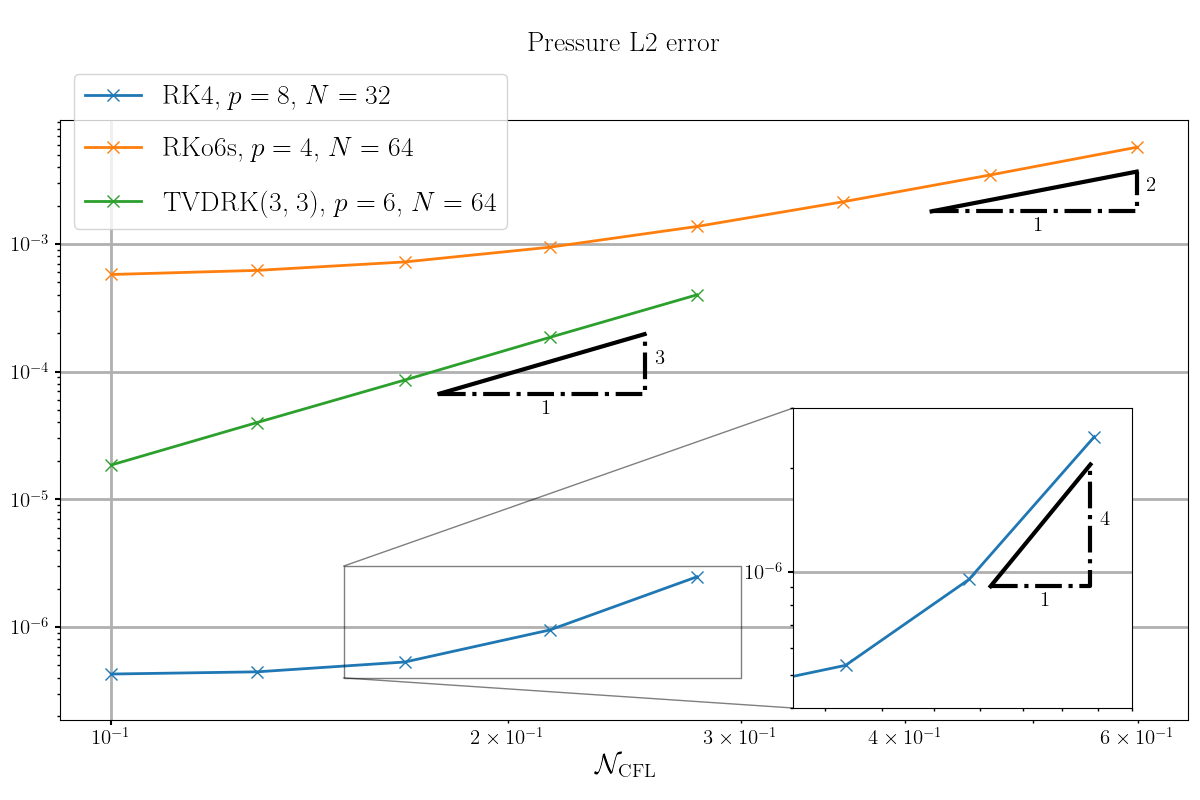
\includegraphics{figures/covo_rk.png}
        \caption{Global truncation error for the RK4, RKo6s and TVDRK(3, 3) methods.}
        \label{fig:covo_rk}
      \end{figure}

      \paragraph{}
      Now that we tried our analysis on traditional explicit Runge--Kutta methods, we look at the newly added exponential Rosenbrock methods.
      Their corresponding error curves are shown in figure \ref{fig:covo_exp}.
      As expected, we see the respective 2, 3 and 4 slope values.
      Furthermore, by looking at the abscissa ranges, we see that they work correctly with higher CFL numbers than all the explicit methods we tried.
      The goal of this first analysis of the exponential integration methods is not to analyse their robustness, but it already seems better than with explicit methods.
      What is interesting from this analysis is that we are able to use higher-order methods with fewer Runge--Kutta stages.
      Furthermore, the additional computational cost of the additional stages is low.
      As we discussed earlier, we can reformulate exponential Rosenbrock methods as in equation (\ref{eq:exprb_defect})  using the defects $D_{n, i}$.
      The first stage of an exponential Rosenbrock method is then an exponential Rosenbrock--Euler method, for which we compute the contribution of the "full" right-hand side $f\left(y_n\right)$.
      Here, this is done with the algorithms previously described, using a Krylov subspace of dimension 20.
      Then, because the defects are relatively smaller, the other stages compute their contribution with only 5 Krylov basis vectors.
      The two exponential Rosenbrock methods with two stages are not a lot more expensive than the Rosenbrock--Euler method.
      In comparison, a 2-stage explicit Runge--Kutta method will be twice as computationally expensive as the Euler method.
      We also tried this analysis with larger Krylov subspace methods.
      In this other configuration, the first stage uses 40 Krylov basis vectors for all three exponential methods, and the second stage uses 10 Krylov basis vectors for the ExpRB32 and ExpRB42 methods.
      However, using a larger subspace did not have any impact on the result of this analysis.
      For all $\left(N, p\right)$ configurations, the error curve as a function of the time step was almost the same as with smaller Krylov subspace, such as they were almost indistinguishable when plotted in figures like figure \ref{fig:covo_exp}.

      \begin{figure}
        \centering
        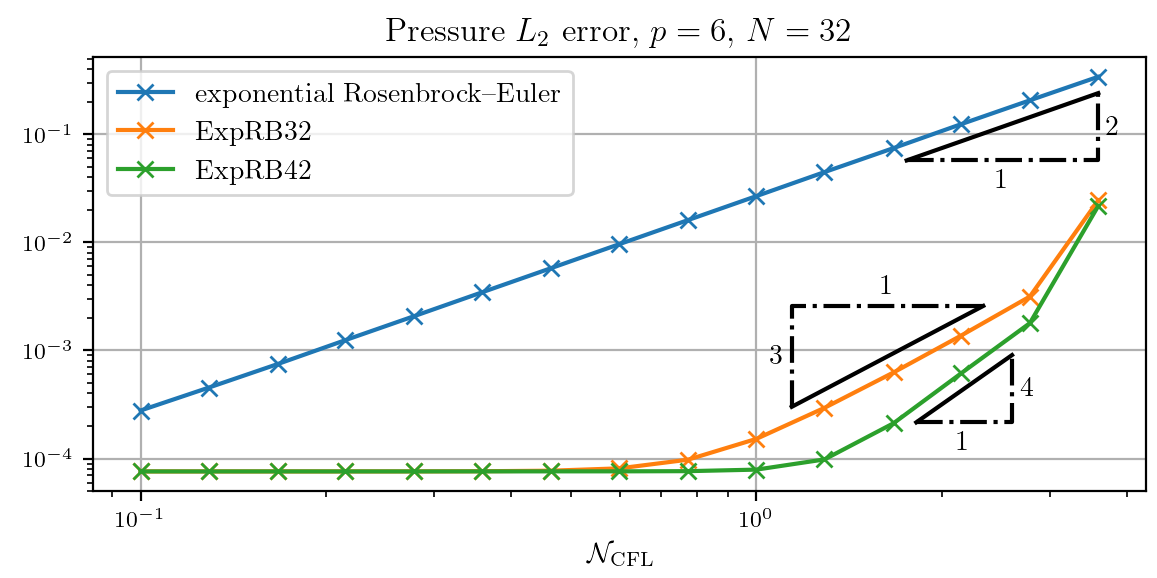
\includegraphics{figures/covo_exp.png}
        \caption{Global truncation error for the exponential Rosenbrock--Euler, ExpRB32 and ExpRB42 methods.}
        \label{fig:covo_exp}
      \end{figure}

      \paragraph{}
      We choose this first test case as it is widespread in the computational fluid dynamic community, as a tool to analyse the order of integration schemes.
      Often, it concerns spatial discretisation methods, but we used it for our time integration method as it gives us easy access to the global truncation error, which is the error that interest the solver users.
      First, we showed that this analysis recover the correct slope on the error curve as a function of the time step for the already existing explicit Runge--Kutta integration methods.
      Indeed, the error converges, as the time step decreases, to a minimum error value that comes from the spatial discretisation scheme.
      By refining the mesh and using higher-order spatial discretisation methods, we are able to reduce this minimal error and observe the expected curve for almost all methods.
      The same analysis but with the newly implemented exponential Rosenbrock methods showed that we get the expected order.
      It also showed that the additional cost of using more stages with exponential methods is relatively small compared to the same additional cost for explicit Runge--Kutta methods.
      Finally, it showed that for this convected inviscid isentropic vortex case, the exponential Rosenbrock methods were much more robust, as they work with higher CFL numbers.
      The analysis of their stability is the topic of the next section.


    \subsection{Robustness: Taylor--Green vortex}
    \PS{Renommer en "Stability: Taylor--Green vortex" ?}

      \paragraph{}
      For the next text case, we choose another explicit computation: the Taylor--Green vortex.
      It is a three-dimensional case where we solve the Navier-Stokes equations in a periodic box of length $2 \pi L$ centered around the origin.
      The initial flow is given by:
      \begin{equation}\label{eq:tgv}
        \left\{\begin{aligned}
          \vec{u} &= \operatorname{Ma} \sqrt{\gamma r_\textrm{gas} T_\infty} \begin{pmatrix}
            \sin\left(\frac{x}{L}\right) \cos\left(\frac{y}{L}\right) \cos\left(\frac{z}{L}\right) \\[10pt]
            \cos\left(\frac{x}{L}\right) \sin\left(\frac{y}{L}\right) \cos\left(\frac{z}{L}\right) \\[10pt]
            0
          \end{pmatrix} \\[10pt]
          T &= T_\infty \\[10pt]
          P &= P_\infty \left(1 + \frac{\gamma \operatorname{Ma}^2}{16} \left(\cos\left(\frac{2x}{L}\right) + \cos\left(\frac{2y}{L}\right)\right) \left(\cos\left(\frac{2z}{L}\right) + 2\right) \right)
        \end{aligned}\right.
      \end{equation}
      over the domain $\left(x, y, z\right) \in \left[-\pi L, \pi L\right]^3$, and can be seen in figure \PS{TODO}.
      Even if $\vec{u}_z = 0$ at the initialisation, it becomes non-null afterwards and the problem is fully three-dimensional.
      The initial flow transition to turbulence: the initial large scales decay into smaller ones, that end up dissipated.

      \paragraph{}
      \PS{UNITÉS ?}
      The numerical values we took in this test case are $L = 1$, $\operatorname{Ma} = 0.1$, $r_\textrm{gas} = 71.4284$, $T_\infty = 1$ and $P_\infty = 71.4288$.
      Because here the fluid viscosity is constant with $\mu = \num{6.25e-4}$, we have the Reynolds number based on L: $\operatorname{Re} = \rho_\infty U\infty L / \mu = 1600$, which is a standard value in many validation cases from the literature \PS{REFs}.
      The Prandtl number, ratio of momentum diffusivity to thermal diffusivity, is equal to 0.71.
      Using the convective time $t_c = L / U_\infty$ \PS{c'est bien ça ?}, it is known for our numerical values that the maximum of dissipation happens around $8 t_c$, and after $15 t_c$ the flow is fully turbulent without any trace of the initial structures.

      \paragraph{}
      The values of interest for this test case are the \PS{mean turbulent kinetic energy averaged over the computational domain $\Omega$}:
      \begin{equation} \PS{TODO}
        E_k = \frac{1}{\Omega} \int_\Omega \rho \frac{\norm{\vec{u}}^2}{2} \mathrm{d}\Omega \ ,
      \end{equation}
      the mean enstrophy, defined by
      \begin{equation} \PS{TODO}
        \mathcal{E} = \frac{1}{\rho_\infty \Omega} \int_\Omega \rho \frac{\norm{\nabla \times \vec{u}}^2}{2} \mathrm{d}\Omega \ ,
      \end{equation}
      and the kinetic energy dissipation rate, that follows the relation:
      \begin{equation} \PS{TODO}
        \epsilon = -\frac{\mathrm{d} E_k}{\mathrm{d} t} = 2 \mu \mathcal{E} \ .
      \end{equation}
      We can compare those values computed by our simulation with some reference values.
      Those reference values were computed using spectral methods derived specially for this Taylor--Green vortex case \PS{Guillaume, c'est bien ça ? Ref ?}.

      \paragraph{}
      The mesh used here is the same for all computations: a regular Cartesian mesh made of $80^3$ cells.
      We use the Spectral Difference method with the order $p = 4$.
      Each computation is run on 308 CPU cores.
      What interest us is that the result from the simulation matches reference data, and how much CPU time the computation took.
      For each time integration method we want to try, we simulate the flow from the initial condition up to $20 t_c$.
      We will work with the RKo6s, TVDRK(3, 3) and SSPRK(5, 4) methods as the already existing reference methods, and the exponential Rosenbrock--Euler and ExpRB32 methods as the newly implemented methods.
      For the exponential Rosenbrock methods, we use Krylov subspaces of dimension 20 for the first stage, and of dimension 5 for the additional stages for the ExpRB32 method.
      We use constant time steps in a simulation, and we try to find the highest time step compatible with the method.
      However, after finding the largest acceptable time step value for the exponential Rosenbrock--Euler method, we tried to increase it.
      To do so, we had to increase the dimension of the Krylov subspaces used to compute $\varphi$-functions.
      By doing so, the computational cost of a single iteration is higher, but it reduces the error in the $\varphi$-functions evaluations and we hope this will help the time integration method.
      Symmetrically, we tried to reduce the dimension of the Krylov subspaces.
      It means that the method can not work with the same time step as before as it is now too high, but this reduces the iterations cost.
      Here we wanted to see if making more iterations that are less expensive can be a good idea.
      We will call ExpEuler($k$) method the exponential Rosenbrock--Euler method that uses a Krylov subspace of dimension $k$.

      \paragraph{}
      The result of all simulation is shown in figure \PS{TODO}.
      As a simulation correspond to the computation with the largest time step for which the results are satisfying, this figure does not gives much information: all methods produce results that are close to reference data.
      The ExpRB42 method is not shown, as it is similar to the ExpRB32 method.
      Indeed, we compare methods that give similar physical results, and what interest us is their statistics.
      As those two methods run at the same highest CFL number and have a similar iteration cost, they behave similarly in this analysis.

      \begin{table}
        \center
        \begin{tabular}{c|cccc}
          Method       & $\mathcal{N}_\textrm{CFL}$ & $N_\textrm{iterations}$ & Time / iteration (s) & Total time (hh:mm:ss) \\ \hline
          RKo6s        & 0.28                       & 50000                   & 1.588                & 22:03:20              \\
          TVDRK(3, 3)  & 0.14                       & 100000                  & 0.833                & 23:08:20              \\
          SSPRK(5, 4)  & 0.28                       & 50000                   & 1.497                & 20:47:30              \\ \hline
          ExpEuler(10) & 1.4                        & 10000                   & 3.803                & 10:33:50              \\
          ExpEuler(20) & 2.8                        & 5000                    & 8.144                & 11:18:40              \\
          ExpEuler(40) & 5.6                        & 2500                    & 19.491               & 13:32:07              \\
          ExpEuler(80) & 11.2                       & 1250                    & 52.792               & 18:19:50              \\
          ExpRB32      & 2.8                        & 5000                    & 10.391               & 14:25:55              \\
        \end{tabular}
        \caption{
          Statistics for various time integration methods.
          Time corresponds to elapsed real time, or wall-clock time.
          A computation corresponds to the simulation of the Taylor--Green vortex from equation (\ref{eq:tgv}) on time interval $\left[0, 20 t_c\right]$.}\label{tab:tgv}
      \end{table}

      \paragraph{}
      In table \ref{tab:tgv}, we show the statistics for each time integration method.
      As the cost of the algorithms used in the time integration methods does not change between iterations, we can compute an average elapsed real time per iteration for each method.
      Among the explicit methods, we see that the RKo6s and SSPRK(5, 4) methods run at a higher CFL number than the TVDRK(3, 3) method.
      However, they have more stages per iteration so each iteration takes longer, and the total elapsed real time is similar between all three methods.
      We note that the cost of one step of an explicit Runge--Kutta method is not proportional to the number of stages.
      Indeed, the implementation of the RKo6s method uses the fact that it is a low storage method to reduce the computational cost in terms of both time and memory.
      Nevertheless, the cost of an iteration of those explicit methods is much less than exponential methods.






    \subsection{Industrial application: LS89}
